\documentclass[12pt]{amsart}
\usepackage[english]{babel}
\usepackage{graphicx}
\usepackage{float}
\usepackage{mathtools}
\usepackage{amsfonts}
\usepackage{amssymb}
\usepackage{siunitx}
\usepackage{amsthm}
\usepackage{enumitem}
\usepackage{stmaryrd}
\usepackage{multirow}
\usepackage[backend=bibtex,style=numeric]{biblatex}
\bibliography{Biblio}
\usepackage[a4paper, total={6in, 10in}]{geometry}
\graphicspath{{./}{}}% You can add the path for the images in the empty brackets 
\title{Study of Electrostatics: Generation and Measurement of Charge}
\author{Josh Goldfaden, Daniel Briseno}
\date{}
\newdimen\graph
\graph=4.2in
\newdimen\medgraph
\medgraph = 5.3in
\newdimen\smallgraph
\smallgraph = 3in
\newdimen\tinygraph
\tinygraph = 1.5in
\renewcommand{\arraystretch}{1.5}
\begin{document}
\maketitle
\section{abstract}
In this set of experiments, the flow of electric charge was studied through initially conducting demonstrations with charge generator machines. In particular, a Van de Graaff Generator was used to illuminate a neon light bulb without making direct contact. This observation demonstrated that there is a flow of electric charge between the generator and the bulb. When bringing a neutrally-charged conductive strip or a ball into close proximity with the generator, the two objects attracted. However, once the two objects made contact, they repelled one and another. Once the objects made contact, charge was transferred from the generator to the object, thus the like charges repelled. Further, when an Electric Plume was placed on the generator, the ribbons threaded through the top of the Electric Plume slowly began to rise and repel one another and the plume as all acquired charge from the generator. The electrostatic force emitted by the generator also induced the movement of the Electric Whirl Spin when brought into close proximity. Another electrostatic machine studied was the Wimshurst Influence Machine. When this machine was cranked, an electric charge was generated and was visible as a spark between the two terminals. The presence of an electric charge was also observed through the use of an electroscope; in particular, the two strips of metal concealed within the apparatus repelled one another when a charged object was brought into contact with a wire suspending each strip. Aside from these apparatuses, various objects (e.g. pieces of metal, wool/fur, glass, wood, etc.) were charged by being rubbed together, and these charges were measured using a Vernier Charge Sensor integrated with a Faraday Pail. From this, it was determined that ----. Further, this apparatus was used to measure the quantity of charge that resides in an individual’s body. It was observed that ----- when an individual scuffed their shoes on a piece of carpet.
 
\section{Introduction}
Electrostatics is a fundamental branch of physics that examines stationary electric charges that generate an electrostatic field. In this particular investigation, an array of apparatuses are utilized to observe the generation of an electrostatic field. One paramount exemplar of such a device is the Van de Graaff generator rendered in Figure 1.\\
\begin{figure}[h]
	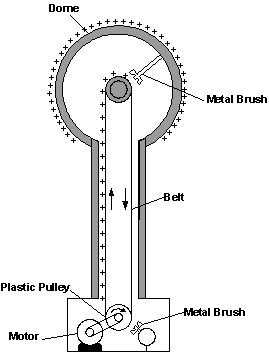
\includegraphics[width=\smallgraph,scale=0.01]{Van.png}
	%h (here) - same location
	%t (top) - top of page
	%b (bottom) - bottom of page
	%p (page) - on an extra page5
	%! (override) - will force the specified location
	\caption{The basic structure of a Van de Graaff generator. Photo Credit  \cite{Vander}}
	\label{Van}
\end{figure}

\indent Within the generator, a moving belt is wound around a plastic pulley. When the motor is in use, it rotates the pulley, which consequently rubs against the belt and induces its motion. The contact between the belt and the pulley results in the generation of static electricity. Particularly, negative charges from the belt is transferred to the plastic pulley.  This acquisition of charge by the pulley is the triboelectric effect in action. That is, two dissimilar objects, the belt and the pulley, come into contact with one another, and the pulley acquires a charge when separated from certain regions of the belt that it was previously in contact with \cite{Vander:2}. As the pulley becomes more negatively charged, it induces a positive charge within the metal brush at the base of the generator through frictional contact. Specifically, the negatively charged pulley is in close proximity to the neutrally charged metal brush. The charged pulley drives the redistribution of electric charge in the metal brush such that the brush acquires a positive electric charge. In essence, an electrostatic field is generated between the plastic pulley and the metal brush, thus causing the air surrounding the brush within the base of the generator to become ionized. The positive charges of the air repel the positively charged brush and accumulate on the surface of the moving belt. These positive charges are subsequently moved by the belt to the dome of the generator. The positive charges on the belt are transferred to the dome via air ionization and the metal brush suspended within the dome. This results in the collection of  positive charge on the surface of the dome, thus increasing its electric potential. Conversely, the Van de Graaff generator can also become negatively charged, depending on the material of the belt and the pulley.\\

\indent In an instance of a negatively charged Van de Graaff generator, the electrons spread across the dome repel one another. When a neon light bulb is brought in proximity to the dome, the electrons are attracted to the anode (the positively charged electrode) of the light bulb\cite{scienceworld}. This movement of electrons results in an electric current between the dome of the generator and the bulb, thus inducing the bulb’s illumination. Additionally, the individual holding the bulb also assists electron flow. Another accessory to the Van de Graaff generator that can be used to observe electrostatics is an Electric Plume, which is mounted on a generator in Figure 2.\newpage
\begin{figure}[h]
	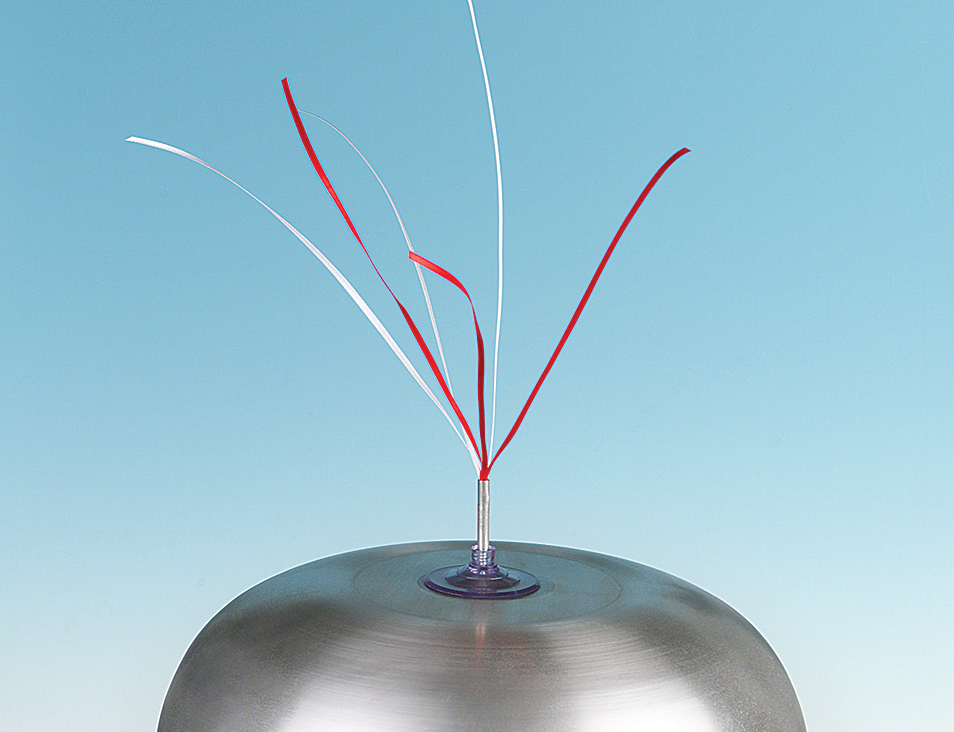
\includegraphics[width=\smallgraph,scale=0.01]{Plume.png}
	%h (here) - same location
	%t (top) - top of page
	%b (bottom) - bottom of page
	%p (page) - on an extra page5
	%! (override) - will force the specified location
	\caption{ An Electric Plume mounted on the dome of a Van de Graaff generator. Photo Credit \cite{Flinn}}
	\label{Plume}
\end{figure}

\indent Electrons are transferred from a negatively charged dome onto the neutrally charged ribbons of the plume. As the ribbons acquire like charges, they begin to repel one another and appear to be suspended in the air as visualized in Figure 2. Electrons that accumulate on the dome of the Van de Graaff generator are also responsible for driving the movement of the Electric Whirl Spin, which is depicted in Figure 3.\\

\begin{figure}[h]
	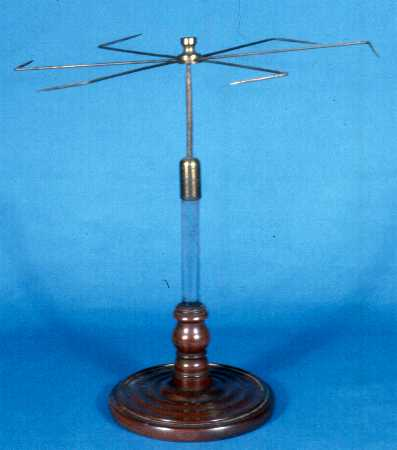
\includegraphics[width=\smallgraph,scale=0.01]{Whirl.png}
	%h (here) - same location
	%t (top) - top of page
	%b (bottom) - bottom of page
	%p (page) - on an extra page5
	%! (override) - will force the specified location
	\caption{One variant of the Electric Whirl Spin. Photo Credit \cite{greenslade}}
	\label{Whirl}
\end{figure}

\indent When brought in proximity to a negatively charged Van de Graaff generator dome, electrons escape from the dome and accumulate onto the pointed ends of the Whirl Spin’s arms. This causes the air around the pointed ends to become ionized and is thus repulsed by the arms. This repulsion by the arms induces their rotation about the pivot they are attached to. Thus, the Electric Whirl Spin begins to twirl \cite{davis_2012}. \\

\indent When a neutrally charged object, such as a pith ball, is brought in proximity to the dome of  Van de Graaff generator, the two objects will be attracted as observable in Figure 4.\\

\begin{figure}[h]
	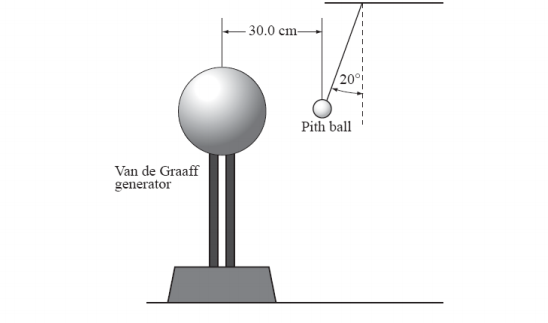
\includegraphics[width=\smallgraph,scale=0.01]{Pith.png}
	%h (here) - same location
	%t (top) - top of page
	%b (bottom) - bottom of page
	%p (page) - on an extra page5
	%! (override) - will force the specified location
	\caption{A neutrally charged pith ball moving towards a charged Van de Graaff generator. Photo Credit \cite{dickie}}
	\label{Pith}
\end{figure} 

\indent This attraction between these two objects is the result of electrostatic induction in that equal amounts of positive and negative charge on the ball are redistributed. For instance, a positively charged Van de Graaff generator will attract the negative charge on the pith ball, thus causing this charge to accumulate on the side of the ball facing the generator. As for the positive charge on the pith ball, this is repelled by the like charged generator thus it accumulates on the side of the ball that is furthest from the generator. However, once the pith ball makes physical contact with the generator, positive charge from the generator is transferred to the ball, thus causing the two objects to repel. 

Another electrostatic generator utilized in this lab is the Wimshurst influence machine, which is depicted in Figure 5. \\
\begin{figure}[h]
	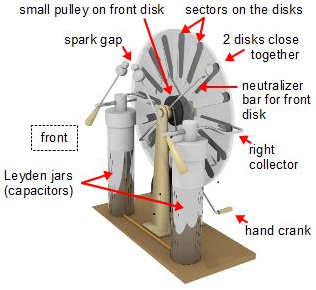
\includegraphics[width=\smallgraph,scale=0.01]{Wim.png}
	%h (here) - same location
	%t (top) - top of page
	%b (bottom) - bottom of page
	%p (page) - on an extra page5
	%! (override) - will force the specified location
	\caption{Wimshurst influence machine components from the front. Photo Credit \cite{Wim}}
	\label{Wim}
\end{figure} 

\indent Unlike the mechanism of the Van de Graaff generator, the Wimshurst influence machine does not rely on friction. Rather, similar to the interaction between a charged Van de Graaff generator and a pith ball depicted in Figure 4, the Wimshurst influence machine generates electrostatic charge through induction. Specifically, the triboelectric effect must be used to induce a charge on the sectors of either disk. Once there is an imbalance in the charge between each disk, the disks can be rotated through manually operating the crank. This crank drives the motion of a pulley system that induces the rotation of the disks. One of the pulley’s belts is twisted causing one disk to spin in the opposite direction of the other disk. Each disk’s sectors have either an excess of positive or negative charge. As the disks rotate, induction occurs between the sectors on each disk. For instance, a negatively charged sector induces the adjacent sector on the neighboring disk. The side of the adjacent sector that is closest to the negatively charged sector accumulates positive charge. The negative charge on this sector is simultaneously repelled and travels along a diagonally positioned neutralizer that is in contact with another sector on the same disk. This repelled negative charge travels to the sector, which causes induction on the neighboring disk. Overall, repeated induction occurs between the sectors of each disk. The positive and negative charge that accumulates on the individual sectors induce the two collectors that are suspended around the disks at opposite ends. The combs of each collector either accept electrons from negatively charged sectors or donate electrons to positively charged sectors. This exchange of electrons creates an electric field between the collectors and the sectors of the disk. The positive and negative charge that build up in the two respective collectors are distributed to two different Leyden jars. These Leyden jars, which serve as capacitors, are composed of an inner metal cylinder, an insulator, and an outer metal cylinder. The two metal cylinders acquire opposite charges, but no neutralization can occur as the insulator between them prevents the exchange of any charges. Similarly, the spark gap between the two conductors mounted on the Leyden jars also serve as a capacitor where air is an insulator. It is noteworthy that increasing the humidity of the air may result in the leakage of electric charge as water is a good conductor, thus limiting the amount of static electricity generated. An electric field is generated in this gap, and the flow of charged particles creates an electric spark. This results in the neutralization of each Leyden jar, and this cycle repeats itself as the crank is continually spun \cite{rim}. \\

\indent A class of  apparatuses that are utilized to determine the presence of electric charge are known as electroscopes. The variant used in this lab is rendered in Figure 6\\
\begin{figure}[h]
	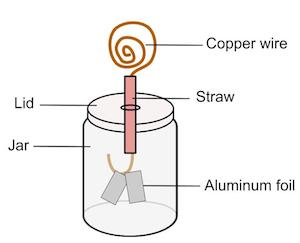
\includegraphics[width=\smallgraph,scale=0.01]{leaf.png}
	%h (here) - same location
	%t (top) - top of page
	%b (bottom) - bottom of page
	%p (page) - on an extra page5
	%! (override) - will force the specified location
	\caption{An aluminum foil leaf electroscope. Photo Credit \cite{Ele}}
	\label{leaf}
\end{figure} 

\indent An object with a suspected static electric charge, such as a balloon that has been rubbed against an individual’s hair, is brought near the copper wire of the electroscope. Electrons from the charged balloon are transferred to the copper wire and flow down the wire. At the end of the wire within the jar, the electrons are finally transferred to the leaves of aluminum foil which consequently gain negative charges. These leaves of negatively charged aluminum foil repel one another, thus indicating the presence of static electric charge on the balloon \cite{Champ}. \\

\indent Interestingly, an individual’s body can also serve as an electrostatic conductor and carries charge. The amount of charge on a human body as well as other suspectedly charged objects can be quantified using a Faraday Pail, a schematic of which is depicted in Figure 7. \\
\begin{figure}[h]
	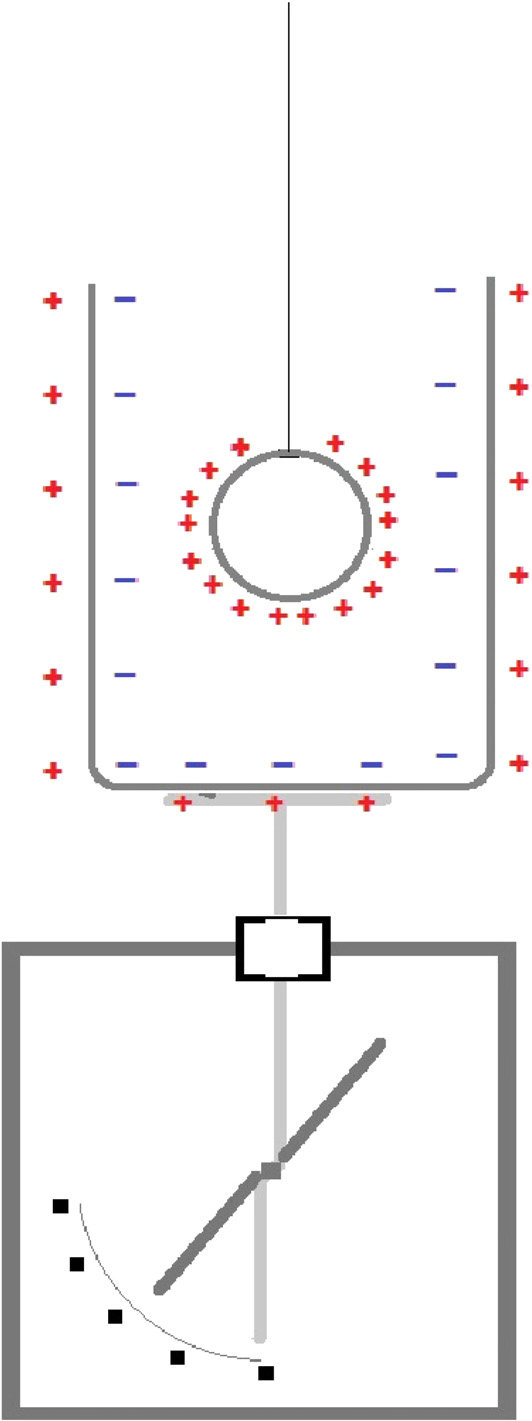
\includegraphics[width=\tinygraph,scale=0.01]{Farday.png}
	%h (here) - same location
	%t (top) - top of page
	%b (bottom) - bottom of page
	%p (page) - on an extra page5
	%! (override) - will force the specified location
	\caption{A diagram of a Faraday Pail integrated with an electrometer.}
	\label{Farday}
\end{figure} 

\indent This apparatus demonstrates that an electric charge encompassed by a conducting shell produces an equal charge on the shell, and the charge of an electrically conducting object resides entirely on its surface. Further, this device also provides a quantification of electrostatic charge. An individual’s body can be grounded and integrated with a ground plane upon which a Faraday Pail sits. When an individual creates a charge by scuffing their shoes on a piece of carpet, this charge can be measured by the device.\\

\indent In this study of electrostatics, we observed the movement of charge between objects by means of friction and induction. In particular, we studied the generation of static electricity using a Van de Graaff generator, a Wimshurst influence machine, and an electroscope. Utilizing a grounded Faraday Pail integrated with a Vernier Charge Sensor, we quantified the charge of various objects as well as our own bodies, which were grounded to the metal plane upon which the Faraday Pail sat. These experiments have provided us an opportunity to not only have a less abstract perception of static electricity, but we have a greater understanding and appreciation for the various physical phenomena that occurs in the world around us.

\section{Electrostatic Experiments}
\indent In this set of experiments, we wanted to further study and quantify the electrostatic charges that exist upon various objects, including our bodies. As humidity influences the flow of charge, we measured the relative humidity of the lab at 51.66\%. In order to measure electrostatic charge, we placed the cage encompassing the Faraday Pail on top of a metal grounding plane, and measured the charge of the pail (and thus indirectly measured the charge of anything placed in the pail). See figure 8 for more details. \\


\begin{figure}[h]
	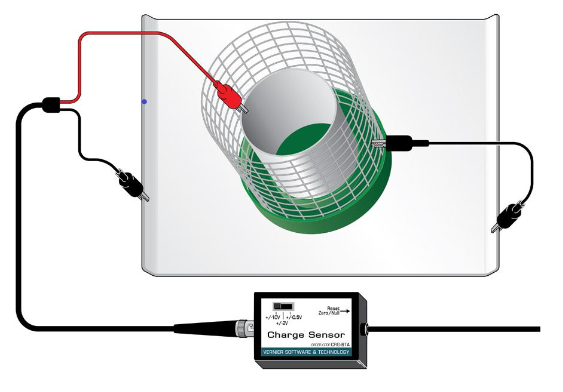
\includegraphics[width=\medgraph,scale=0.01]{FardaySetup.png}
	%h (here) - same location
	%t (top) - top of page
	%b (bottom) - bottom of page
	%p (page) - on an extra page5
	%! (override) - will force the specified location
	\caption{Faraday Pail Setup. The charge sensor is set to $\pm$10 V}
	\label{FardaySetup}
\end{figure} 

\subsection{Measuring Charge on Our Own Bodies}
\indent We first attempted to measure the charge of our own hands by inserting our finger into the Faraday Pail. Our procedures for this part of the experiment can be summarized as follows:
\begin{enumerate}
	\item Scuff shoes on laboratory floor.
	\item Insert a finger into the pail without touching the pail or cage and record charge sensor readings.
	\item Remove finger from pail and record charge sensor readings
	\item Touch the metal grounding plate with your finger, then repeat steps (2) and (3).
	\item Ground the alligator clip on the grounding strap to the grounding plate and attach grounding strap to wrist.
	\item Repeat steps (1)-(4)\\
\end{enumerate}

\indent Unsurprisingly, none of the measurements taken while wearing the grounding straps showed a significant change in charge when we inserted a finger in the Faraday Pail. This can be attributed to the fact that the grounding strap ensures that our bodies have the same electric charge as the grounding plate, and thus should cause no change in the charge of a neutral pail.\\
\indent However, the measurements taken without wearing the grounding strap showed no significant changes in the charge of the pail as well. While this somewhat surprising considering that we were not grounded when making these measurements, it may be explained by 2 factors: 1 -- the relatively high humidity in the lab may have been enough to discharge our bodies to the surrounding air, making us more or less continuously grounded; 2 -- the sensor gave readings varying from 0-30nC even after grounding the pail and keeping the pail empty (such that the reading should have been 0nC), showing that the sensor may not have been giving accurate data and thus masked a significant change in charge. 

\subsection{Separation of Charge}
\indent After measuring the electrostatic charge on our own bodies, we measured the charge obtained by different material when rubbed against a dissimilar object. We rubbed a wooden rod, a PVC rod, and a nylon rod against Vinyl, Felt, and a cotton washcloth. We then measured the charge obtained by the rods after being rubbed with the different materials:
\begin{table}[H]
	\begin{tabular}{ |c|c||c|c|}
		\hline
	
		\hline
		Rod Material & Material rubbed on rod& Type of charge (+,0,-)&Amount of Charge (nC)\\
		\hline
		\multirow{3}{*}{Wooden Rod} &Vinyl&0&0\\
		 &Felt&0&0\\
		&Washcloth&0&0\\
		\hline	
		\multirow{3}{*}{PVC Rod}&Vinyl&-&24.80\\
		&Felt&-&33.00\\
		&Washcloth&-&14.40\\
		\hline
		\multirow{3}{*}{Nylon Rod} &Vinyl&+&5.00\\
		&Felt&-&1.30\\
		&Washcloth&0&0\\
		\hline	
	\end{tabular}
\caption{Charge obtained by various rods after rubbing on different materials}
\end{table}

\indent As seen in Table 1, the wooden rod, even when rubbed with a sheet of vinyl, felt, and a washcloth, failed to obtain a charge. One may speculate that the wooden rod's inability to hold an electrostatic charge is due to wood being a poor conductor. Atomically speaking, the electrons of the atoms that compose the wooden rod are unable to move freely such that they can generate an electrical charge. However, the PVC rod and the Nylon rod were both able to hold a charge, and both are also poor conductors.\\
\indent Unlike the nylon and PVC rods, the wooden rod was quite porous. The presence of air within the rod may have allowed the wooden rod to discharge into the environment, as well as limiting the amount of surface area in contact with the rubbing fabrics. Therefore, we believe that the wood's inability to hold an electrostatic charge was due to the wood being porous rather than a bad conductor.\\

\indent With respect to the charges measured that correspond to the PVC rod being rubbed with the materials listed previously, it is observable that the PVC rod acquired a negative charge after being rubbed by all 3 types of fabrics. However, the amount of charge deposited on the PVC rod by the different fabrics was different, with the felt depositing the most and the washcloth the least.
 
\indent Regarding the charges measured that correspond to the nylon rod being rubbed with these same materials, it was found that when rubbed with vinyl, the rod acquired a small positive charge. When rubbed with felt, the nylon rod acquired a small negative charge. When rubbed with a washcloth, the nylon rod remained neutral in charge.\\

\indent Recall from the introduction that the triboelectric effect (the separation of charge caused by rubbing two dissimilar objects together) is a result of small chemical interactions between the dissimilar objects being rubbed. More specifically, when two dissimilar objects are brought into contact there are some chemical bonds formed between negatively charged regions of one object and positively charged regions of the other. Because of these chemical bonds, some negative charge is ''pulled" from one object to the other, leaving the ''pulling" object negatively charged and the other positively charged. Since chemical interactions are a result of \textit{both} object's atomic structure, it makes sense that the PVC, wood and nylon rods all reacted differently to the different rubbing materials and that in some cases, each rod acquired different charges from the three materials.\\

\indent During this experiment we also attempted to measure the charge separation created by: taking two tapes, taping one to a table and taping the other on top of the first, quickly taking both tapes off the table, then quickly separating the two tapes. Indeed, the tapes acted as if at least one of them was charged since there was an observable attractive force between them. However, we were unable to measure any charge using the Faraday Pail apparatus. Provided the relative humidity percentage and sensor inaccuracy mentioned previously, it is unsurprising that the charge of both the T Strip and the B Strip was unable to be determined.
\newpage

\printbibliography

	
\end{document}